\chapter{Theory}\label{chap:Theory}
    In this chapter, the theoretical motivation of a search for \HpmLong is described. Firstly, a review of the Standard Model of particle physics (SM) is laid out, then a brief overview of Supersymmetry focusing on the Minimal Supersymmetric Standard Model (MSSM). Finally, the Type II 2-Higgs Doublet Model's (2HDM) relation to the \Hpm production cross section and subsequent branching ratio into SM particles is described as motivation for the choice of studying \HpmLong.

\section{The Standard Model}\label{sec:SM}
	 The SM of particle physics is a quantum field theory that describes all known matter and forces. The SM is built upon a gauge group of type $SU(3)_C \times SU(2)_L \times U(1)_Y$. The $SU(3)_C$ term dictates the strong interaction while the $SU(2)_L \times U(1)_Y$ term describes the electroweak interaction. These interactions occur between fundamental particles called fermions that comprise the known matter of the universe. The interactions, or forces, are mediated by fundamental particles called bosons. 

	\subsection{Particles}\label{ssec:Particles}
		The particles that make up the SM are separated into two groups according to their intrinsic angular momentum charge, or spin. Fermions are those that carry half-integer spin, and thus obey Fermi-Dirac statistics, while Bosons carry full integer spin values and obey Bose-Einstein statistics.
		
		\subsubsection{Fermions}\label{sssec:Fermions}
			The matter we encounter in everyday life is comprised of fermions. Fermions are subdivided into two groups, quarks and leptons. The quarks participate in the strong interaction via their color charge. Quarks cannot exist as a singular particle and thus combine into hadrons in a process called hadronization; the bound states they form are colorless. The proton and neutron are examples of hadrons. Leptons carry no color charge and therefore do not participate in strong force interactions. The fermions in the SM all participate in the electroweak interaction. However, the electromagnetic interaction is limited to those fermions that carry an electromagnetic charge. Section \ref{sssec:ElectroWeak} describes the electroweak interaction in detail.

			Fermions can then be further divided into three generations, each lepton has an electrically neutral weak force partner in the form of a neutrino. Table~\ref{tab:fermions} lists all the SM fermions and their properties.


			\begin{table}[!thp]
				% \centering
				\caption{Standard Model fermions and their properties ~\cite{pdg}}
				\resizebox{\textwidth}{!}{\begin{tabular}{c | c | c | c | c | c | c | c |}
				\cline{2-8}

																& \begin{tabular}[c]{@{}c@{}}$1^{st}$ \\ Generation \end{tabular} & \begin{tabular}[c]{@{}c@{}} $2^{nd}$ \\ Generation \end{tabular} 	& \begin{tabular}[c]{@{}c@{}} $3^{rd}$ \\ Generation \end{tabular}	& Spin 			& \begin{tabular}[c]{@{}c@{}}EM \\Charge \end{tabular}		& Color 		& Mass \\[1ex] \hline
				\multicolumn{1}{|c|}{\multirow{3}{*}{Quarks}}   & Up (u)						& Charm (c)						& Top (t)						& $\frac{1}{2}$ & $+\frac{2}{3}$	& \scalecheck  	& \begin{tabular}[c]{@{}c@{}} $m_u = 2.16^{+0.49}_{-0.26}$ MeV \\[1ex] $m_c = 1.27 \pm 0.02$ GeV \\[1ex] $m_t = 172.76 \pm 0.30$ GeV \end{tabular}		\\[1ex] \cline{2-8}
				\multicolumn{1}{|l|}{}                         	& Down (d)						& Strange (s)					& Bottom (b) 					& $\frac{1}{2}$ & $-\frac{1}{3}$	& \scalecheck	& \begin{tabular}[c]{@{}c@{}} $m_d = 4.67^{+0.48}_{-0.17}$ MeV \\[1ex] $m_s = 93^{11}_{-5}$ MeV \\[1ex] $m_b = 4.18^{0.03}_{-0.02}$ GeV \end{tabular}				\\[1ex]	\hline
				\multicolumn{1}{|c|}{\multirow{3}{*}{Leptons}}  & Electron ($e^{-}$)			& Muon ($\mu^{-}$)				& Tau ($\tau^{-}$)				& $\frac{1}{2}$ & $-1$ 				& X 			& \begin{tabular}[c]{@{}c@{}} $m_{e^{-}} = 0.51$ MeV \\[1ex] $m_{\mu^{-}} = 105.65$ MeV \\[1ex] $m_{\tau^{-}} = 1776.86 \pm 0.12$ MeV \end{tabular}		\\[1ex] \cline{2-8}
				\multicolumn{1}{|c|}{}  						& \begin{tabular}[c]{@{}c@{}}Electron \\ Neutrino\end{tabular} ($\nu_{e}$)	& \begin{tabular}[c]{@{}c@{}}Muon \\ Neutrino\end{tabular} ($\nu_{\mu}$)	& \begin{tabular}[c]{@{}c@{}}Tau \\ Neutrino\end{tabular} ($\nu_{\tau}$) & $\frac{1}{2}$ & $0$ 				& X 			& \begin{tabular}[c]{@{}c@{}} $m_{\nu_{e}} < 1.1$ eV \\[1ex] $m_{\nu_{\mu}} < 0.19 $ MeV  \\[1ex] $m_{\nu_{\tau}} < 18.2 $ MeV \end{tabular}		\\[1ex] \hline			
				\end{tabular}}
				\label{tab:fermions}
			\end{table}


		\subsubsection{Bosons}\label{sssec:Bosons}
			Bosons are colloquially referred to as force-carriers in that the fundamental forces act via exchanging gauge bosons. This means that each force has an associated boson which is described by a field theory. The ElectroWeak quantum field theory (QFT) is more complicated, and is described in detail in section~\ref{sssec:ElectroWeak}. Table~\ref{tab:bosons} lists the SM bosons \footnote{excluding the Higgs}, their associated field theory and properties.

			\begin{table}[!thp]
			\centering
			\caption{Standard Model bosons and their properties ~\cite{pdg}}
			\resizebox{\textwidth}{!}{\begin{tabular}{| c | c | c | c | c | c |}  
			\hline
			\multicolumn{1}{|c|}{Field Theory}							& Boson 				& Spin 	& \begin{tabular}[c]{@{}c@{}} EM \\ Charge \end{tabular} 	& Color 		& Mass 	\\[1ex] \hline 
			\multicolumn{1}{|c|}{Quantum Chromodynamics (QCD)}			& Gluon (g)				& 1 	& 0 														& \scalecheck 	& 0		\\[1ex] \hline
 			\multicolumn{1}{|c|}{Quantum Electrodynamics (QED)} 		& Photon ($\gamma$) 	& 1 	& 0 													 	& X 			& $< 1 \, \mathrm{x} \, 10^{-18}$ eV  	\\[1ex] \hline
			\multicolumn{1}{|c|}{\multirow{2}{*}{ElectroWeak Theory}} 	& $W^{\pm}$ 			& 1 	& $\pm 1$													& X 			& $80.379 \pm 0.012$ GeV	\\[1ex] \cline{2-6}
			\multicolumn{1}{|c|}{} 										& $Z^{0}$				& 1 	& 0 													 	& X 			& $91.1876 \pm 0.0021$ GeV  	\\[1ex] \hline
			\end{tabular}}
			\label{tab:bosons}
			\end{table}

	\subsection{Interactions}\label{ssec:Interactions}

		At its core, the SM relies upon symmetries. From these symmetries, conservation laws follow. It is these laws of conservation, and the breaking of tthe associated symmetry, that dictate the allowed interactions of matter. The first, being a symmetry under charge conjugation, mirror reflection, and time reversal is known as CPT symmetry. The symmetry between charge conjugation and mirror reflection (CP) can be broken in certain circumstances, but holds in strong and electromagnetic interactions. This breaking of CP symmetry occurs in the weak interaction and implies a non-symmetry between matter and antimatter. Since this symmetry holds for strong and electromagnetic interactions, baryon number $(B = \frac{1}{3}(n_{q} - n_{\bar{q}}) )$ and lepton number are conserved in SM interactions. Lepton generation number \footnote{Ignoring neutrino oscillations}, electric charge, color charge, 4-momentum ($p=(E,\vec{p})$), and angular momentum are all conserved in the SM.

		\subsubsection{Quantum Electrodynamics}\label{sssec:QED}

		The electromagnetic force is governed by the QFT known as Quantum Electrodynamics (QED). This force is mediated by the photon, $\gamma$, a massless boson with EM charge 0. The EM force only affects, in other words, the photon only interacts with, charged particles; including all quarks and the $e$, $\mu$, and $\tau$ leptons. Antiparticles are those that carry the opposite EM charge from their normal counterparts and differ in no other way. Antiparticles are denoted by a bar above the particle symbol $(e, \bar{e})$.

		\subsubsection{ElectroWeak Interaction}\label{sssec:ElectroWeak}

		The weak force is most often seen in nuclear decays and is mediated by the $W^{\pm}$ and $Z^0$ bosons. Due to the relatively large mass of these bosons, the weak force has a very limited range. The $W^{\pm}$ affects the third component of isospin ($T_3$), thus only coupling to so called left-handed fermions. This ``handedness'', or chirality, is a property similar to color charge, in that an individual particle can have a number of different values. Table~\ref{tab:weak} contains the allowed values for isospin ($T$) and hypercharge ($Y_W$). 

		\begin{table}[!thp]
				\centering
				\caption{Standard Model fermions and their ElectroWeak properties ~\cite{pdg}}
				\resizebox{\textwidth}{!}{\begin{tabular}{| c | c | c | c | c | c | c | c | c | c | c | c |}
				\hline

																& \begin{tabular}[c]{@{}c@{}}$1^{st}$ \\ Generation \end{tabular} & \begin{tabular}[c]{@{}c@{}} $2^{nd}$ \\ Generation \end{tabular} 	& \begin{tabular}[c]{@{}c@{}} $3^{rd}$ \\ Generation \end{tabular}		& \begin{tabular}[c]{@{}c@{}}EM \\ Charge \end{tabular} & \multicolumn{2}{|c|}{$Y_{W}$} & \multicolumn{2}{|c|}{T} 	& \multicolumn{2}{|c|}{$T_{3}$} \\ \hline
				& & & & &  LH 				& RH 					& LH 			& RH 				& LH 	& RH \\ \cline{6-11}
				\multicolumn{1}{|c|}{\multirow{3}{*}{Quarks}}   & Up (u)						& Charm (c)						& Top (t)						&  $+\frac{2}{3}$ & $+\frac{1}{3}$	& $+\frac{4}{3}$		& $\frac{1}{2}$	& 0					& $\pm \frac{1}{2}$	 	& 0	 \\[1ex] \cline{2-11}
				\multicolumn{1}{|l|}{}                         	& Down (d)						& Strange (s)					& Bottom (b) 					&  $-\frac{1}{3}$ & $+\frac{1}{3}$	& $-\frac{2}{3}$		& $\frac{1}{2}$	& 0					& $\pm \frac{1}{2}$	 	& 0	 \\[1ex] \hline
				\multicolumn{1}{|c|}{\multirow{3}{*}{Leptons}}  & Electron ($e^{-}$)			& Muon ($\mu^{-}$)				& Tau ($\tau^{-}$)				&  $-1$ & $-1$				& $0$					& $\frac{1}{2}$	& 0					& $\pm \frac{1}{2}$	 	& 0	 \\[1ex] \cline{2-11}
				\multicolumn{1}{|c|}{}  						& \begin{tabular}[c]{@{}c@{}}Electron \\ Neutrino\end{tabular} ($\nu_{e}$)	& \begin{tabular}[c]{@{}c@{}}Muon \\ Neutrino\end{tabular} ($\nu_{\mu}$)	& \begin{tabular}[c]{@{}c@{}}Tau \\ Neutrino\end{tabular} ($\nu_{\tau}$) & $0$ & $-1$				& $-2$					& $\frac{1}{2}$	& 0					& $\pm \frac{1}{2}$	 	& 0	 \\ \hline			
				\end{tabular}}
				\label{tab:weak}
			\end{table}

		The $W^\pm$ bosons have a $T_3$ component of isospin and act as raising or lowering operators on the $T_3$ component of left handed fermions. The Z does not have a $T_3$ component, and thus does not act on isospin of fermions. However, the Z boson instead transfers momentum, energy, and spin on all fermions irregardless of their chirality. At energies $> 100 $ GeV the electromagnetic and weak forces combine into the electroweak force. In fact, isospin and hypercharge combine to give electromagnetic charge. $Q_{EM} = T_3 + \frac{1}{2} Y_W$

		% \begin{table}[!thp]
		% 	\centering
		% 	\caption{Standard Model particles and their electroweak quantum numbers ~\cite{pdg}}
		% 	\begin{tabular}{| c | c | c | c | c | c | c |}  
		% 	\hline
		% 	Particle 	& \multicolumn{2}{|c|}{$Y_{W}$} & \multicolumn{2}{|c|}{T} 	& \multicolumn{2}{|c|}{$T_{3}$} \\ \hline
		% 				& LH 				& RH 					& LH 			& RH 				& LH 	& RH \\ \hline
		% 	u 			& $+\frac{1}{3}$	& $+\frac{4}{3}$		& $\frac{1}{2}$	& 0					& $\pm \frac{1}{2}$	 	& 0	 \\[1ex] \hline
		% 	d 			& $+\frac{1}{3}$	& $-\frac{2}{3}$		& $\frac{1}{2}$	& 0					& $\pm \frac{1}{2}$	 	& 0	 \\[1ex] \hline
		% 	c 			& $+\frac{1}{3}$	& $+\frac{4}{3}$		& $\frac{1}{2}$	& 0					& $\pm \frac{1}{2}$	 	& 0	 \\[1ex] \hline
		% 	s 			& $+\frac{1}{3}$	& $-\frac{2}{3}$		& $\frac{1}{2}$	& 0					& $\pm \frac{1}{2}$	 	& 0	 \\[1ex] \hline
		% 	t 			& $+\frac{1}{3}$	& $+\frac{4}{3}$		& $\frac{1}{2}$	& 0					& $\pm \frac{1}{2}$	 	& 0	 \\[1ex] \hline
		% 	b 			& $+\frac{1}{3}$	& $-\frac{2}{3}$		& $\frac{1}{2}$	& 0					& $\pm \frac{1}{2}$	 	& 0	 \\[1ex] \hline
		% 	e 			& $-1$				& $0$					& $\frac{1}{2}$	& 0					& $\pm \frac{1}{2}$	 	& 0	 \\[1ex] \hline
		% 	$\nu_e$ 	& $-1$				& $-2$					& $\frac{1}{2}$	& 0					& $\pm \frac{1}{2}$	 	& 0	 \\[1ex] \hline
		% 	$\mu$ 		& $-1$				& $0$					& $\frac{1}{2}$	& 0					& $\pm \frac{1}{2}$	 	& 0	 \\[1ex] \hline
		% 	$\nu_\mu$ 	& $-1$				& $-2$					& $\frac{1}{2}$	& 0					& $\pm \frac{1}{2}$	 	& 0	 \\[1ex] \hline
		% 	$\tau$ 		& $-1$				& $0$					& $\frac{1}{2}$	& 0					& $\pm \frac{1}{2}$	 	& 0	 \\[1ex] \hline
		% 	$\nu_\tau$ 	& $-1$				& $-2$					& $\frac{1}{2}$	& 0					& $\pm \frac{1}{2}$	 	& 0	 \\[1ex] \hline
		% 	$\gamma$ 	& \multicolumn{2}{|c|}{$0$}					& $\frac{1}{2}$	& 0					& $\pm \frac{1}{2}$	 	& 0	 \\[1ex] \hline
		% 	$g$ 		& \multicolumn{2}{|c|}{X}					& $\frac{1}{2}$	& 0					& $\pm \frac{1}{2}$	 	& 0	 \\[1ex] \hline
		% 	$W$ 		& \multicolumn{2}{|c|}{$0$}					& $\frac{1}{2}$	& 0					& $\pm \frac{1}{2}$	 	& 0	 \\[1ex] \hline
		% 	$Z$ 		& \multicolumn{2}{|c|}{$0$}					& $\frac{1}{2}$	& 0					& $\pm \frac{1}{2}$	 	& 0	 \\[1ex] \hline
		% 	$H$ 		& \multicolumn{2}{|c|}{$+1$}				& $\frac{1}{2}$	& 0					& $\pm \frac{1}{2}$	 	& 0	 \\[1ex] \hline
		% 	\end{tabular}
		% 	\label{tab:weak}
		% 	\end{table}

		\subsubsection{Quantum Chromodynamics}\label{sssec:QCD}
		
		Quantum chromodynamics (QCD) is the QFT that describes the strong force that holds together atomic nuclei and other objects called hadrons. The strong force interacts via the color charge \footnote{This color does is not the visual color we are used to. Merely a convenient analogous naming scheme.} which can have values of either red, green, or blue. Particles that have a color charge cannot exist on their own, they must form colorless bound states called hadrons. Since the strong force grows with distance, if a quark is ejected out from a hadron, the stored energy is such that new particles with color charge will be spontaneously created from the vacuum, binding with the free quark in a process called hadronization. In a particle detector, the hadronization process cascades and creates showers of hadrons that are reconstructed as so called jets.

	\subsection{The Higgs Mechanism}\label{ssec:Higgs}

		The Higgs field is the mass generator of the SM and was first theorized by Peter Higgs~\cite{Higgs-paper}, François Englert, and Robert Brout~\cite{Englert-Brout} in 1964.  The SM itself has four massless Goldstone bosons that do not correspond to the observed bosons. Instead, the Higgs mechanism couples to them via a complex scalar doublet. 
		\begin{equation}\label{eqn:scal doub} \phi = \binom{\phi^+}{\phi^0}\end{equation}
		The scalar potential that gives rise to this phenomena can be written as 
		\begin{equation}\label{eqn:higgs potential} V(\phi) = \mu^2 |\phi^{\dagger}\phi| + \lambda (|\phi^{\dagger}\phi|)^2\end{equation}
		When $\mu^2>0$ and $\lambda>0$ the minimum of the potential $V(\phi)$ is 0. 
		\begin{figure}[!ht] \centering 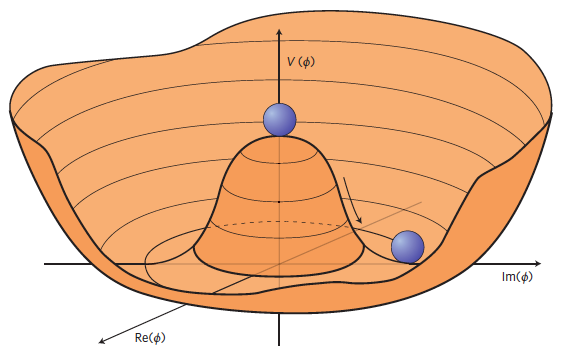
\includegraphics[width=.7\textwidth,keepaspectratio=true]{chapters/chapter2_theory/images/higgspotential.png} \caption{The Higgs potential defined in~\ref{eqn:higgs potential} with $\mu^2<0$ ~\cite{Higgs-phys}} \label{fig:higgs-potential}\end{figure}
		However, when $\mu^2<0$, the scalar potential $V(\phi)$ takes the shape shown in figure~\ref{fig:higgs-potential}
		It follows that the vacuum expectation value (VEV) of $\phi$ is then 
		\begin{equation}\label{eqn:higgs vev} \langle \phi \rangle = \sqrt{\frac{-\mu^2}{2\lambda}} = \frac{\nu}{\sqrt{2}}	\end{equation}
		From here, convention states that we choose an arbitrary direction of the fluctuation as 
		\begin{equation}\label{eqn:phi zero} \phi^0 = \frac{1}{\sqrt{2}} \binom{0}{\nu} \end{equation}
		By choosing these values, $SU(2)$ and $U(1)_Y$ symmetries are broken, the Goldstone bosons are ``eaten'' and we are left with the remaining degree of freedom being the real scalar field $h(x)$
		\begin{equation}\label{eqn:phi-h} \phi(x) = \phi^0 + h(x) \end{equation}
		Substituting in our definition of $\phi^0$, we get
		\begin{equation}\label{eqn:phi-h-vec} \phi = \frac{1}{\sqrt{2}} \binom{0}{\nu+h(x)} \end{equation}
		and couples to the gauge bosons via 
		\begin{equation}\label{eqn:coupling} (\frac{1}{2} g \vec{\sigma} \cdot \vec{W} + \frac{1}{2} g^\prime B ) \phi^0  \end{equation}, where $\vec{\sigma}$ are the Pauli matrices, $\vec{W}$ are $W_{1,2,3}$, $g$ is the weak coupling constant, and $g\prime$ is the hypercharge coupling constant. From this coupling, we get the four eigenstates that correspond to the observed bosons
		\begin{equation}\label{eqn:mass-eigenstates} \begin{split}
		W^\pm = \frac{1}{\sqrt{2}} ( W^1_\mu \mp i W^2_\mu ) \\
		Z^\mu = \frac{ - g\prime B_\mu + g W^3_\mu }{ \sqrt{g^2+g\prime^2} } \\
		A^\mu = \frac{ g B_\mu + g\prime W^3_\mu }{ \sqrt{g^2+g\prime^2} }
		\end{split}
		\end{equation}
		These eigenstates have corresponding mass values of 
		\begin{equation}\label{eqn:mass-eigenstates-masses} \begin{split}
		M^2_W = \frac{1}{4}g^2\nu^2 \\
		M^2_Z = \frac{1}{4}(g^2+g\prime^2)\nu \\
		M^2_A = 0
		\end{split}
		\end{equation}
		The eigenstate labeled here as $A$ is the photon. The Higgs boson was discovered in 2012 by the ATLAS and CMS collaborations at CERN with a mass of $125$ GeV ~\cite{higgs-discovery-atlas}. The scalar boson that was found appears to be the SM Higgs Boson. 

		\begin{figure}[!ht]
		\centering
		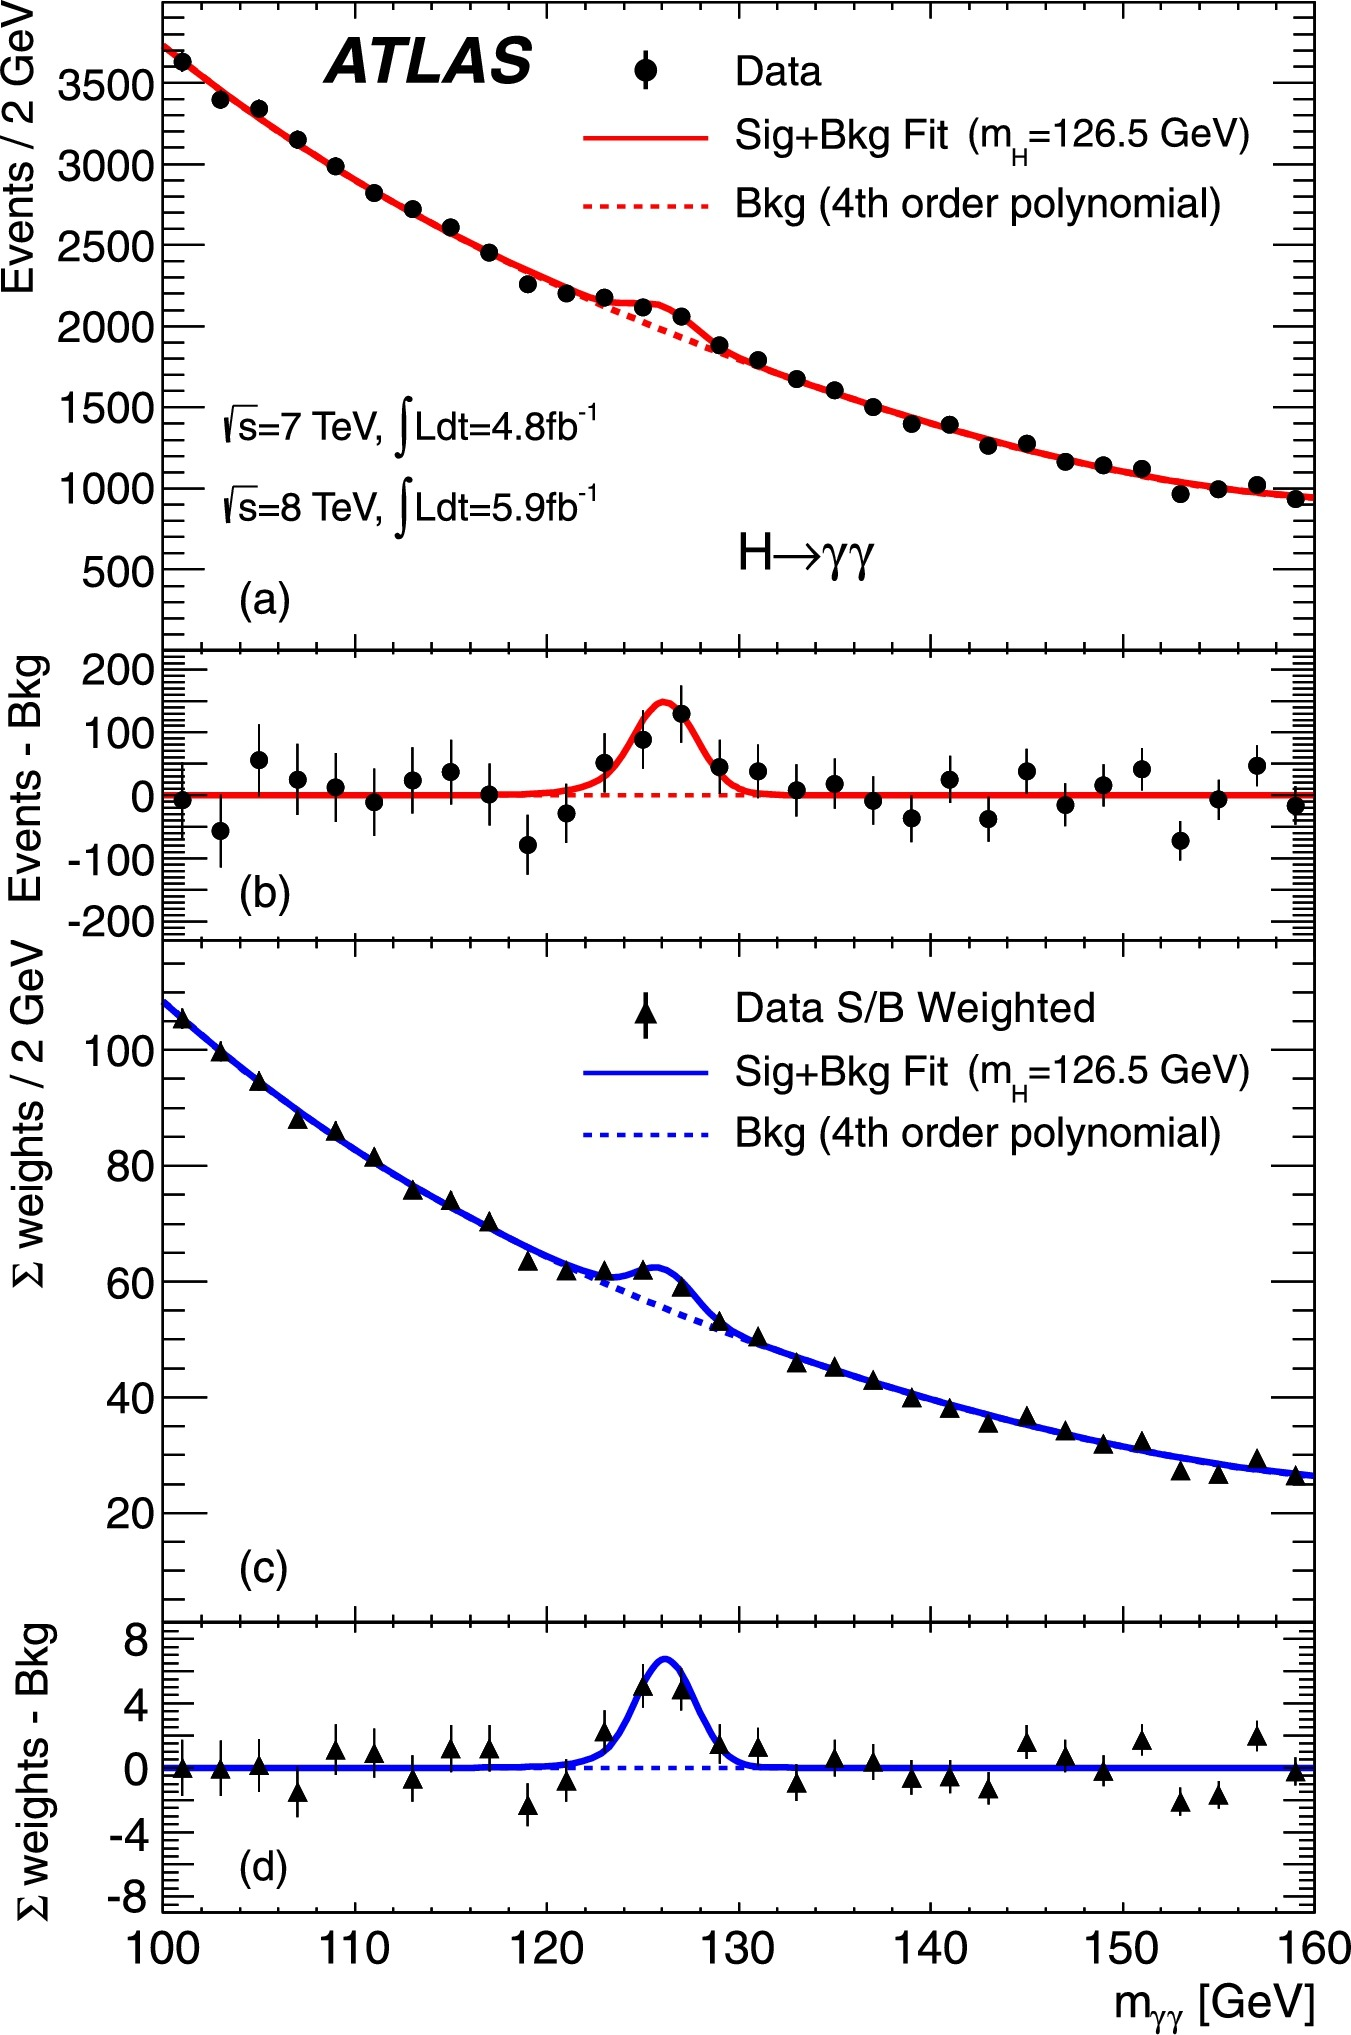
\includegraphics[width=.7\textwidth,keepaspectratio=true]{chapters/chapter2_theory/images/Higgs_Discovery_gam_gam.jpeg}
		\caption{The distributions of the invariant mass of diphoton candidates after all selections for the combined 7 TeV and 8 TeV data sample. The inclusive sample is shown in (a) and a weighted version of the same sample in (c); the weights are explained in the text. The result of a fit to the data of the sum of a signal component fixed to $m_H=126.5$ GeV  and a background component described by a fourth-order Bernstein polynomial is superimposed. The residuals of the data and weighted data with respect to the respective fitted background component are displayed in (b) and (d).}
		\label{fig:higgs-discovery}
		\end{figure}

\section{Supersymmetry}\label{sec:SUSY}
	While the SM is describes a wide range of physics to a high degree of accuracy, it is not without issues. To name a few, gravity, dark matter, and the observed matter-antimatter asymmetry of the universe are not defined by the SM. In addition, the SM defines the mass of neutrinos to be 0. However, because neutrino mixing is observed, where $\nu_e \rightarrow \nu_\mu$ is seen, neutrinos must have mass. 

	One promising model that offers solutions to many of these issues is Supersymmetry (SUSY). As discussed previously, the SM is built upon symmetries, and the breaking of these symmetries gives us electroweak unification. SUSY proposes another symmetry, this time between fermions and bosons. 
	\begin{equation}\label{eqn:SUSY}
	\begin{split}
		Q | Fermion \rangle = | Boson \rangle, \\
		Q | Boson \rangle = | Fermion \rangle
	\end{split}
	\end{equation}
	Equation~\ref{eqn:SUSY} shows how the SUSY operator Q acts on particles.  SUSY naturally offers solutions to the ``hierarchy problem'' with the SM. 

	The hierarchy problem arises from the difference in electroweak ($M_W\sim100$ GeV)  and Planck ($M_P\sim2.4\, \mathrm{x} \, 10^{18}$ GeV) mass scales. For the Higgs mass to be on the scale of $M_H \sim 125$ GeV incredibly large and small mass terms must cancel perfectly, leading to a feeling of ``unnaturalness''. SUSY brings many new particles into the picture, theorized to occupy the intermediate mass range leading to a more natural theory.

	\subsection{MSMM Particles}\label{ssec:MSMM}
		SUSY is a large group of theories, including many additional superpartner particles. The Minimal Supersymmetric Standard Model (MSSM) is the smallest extension of the SM that introduces SUSY. In the MSSM, each SM particle is part of a supermultiplet with it's superpartner where both particles have the same quantum numbers, except spin. If this supersymmetry is unbroken, then the superpartner and the SM particle would have the same mass as well. However, SUSY has not been observed, so the supersymmetry must be broken putting the mass scale on the TeV scale. 

			\begin{table}[!thp]
				\centering
				\caption{SM particles and their MSSM partners~\cite{pdg}}
				\begin{tabular}{| l | c | c |}
				\hline
				Name 				& SM 	& MSSM \\[1ex] \hline
				\multicolumn{3}{|c|}{Spin-$\frac{1}{2}$ quarks and spin-$0$ squarks} \\[1ex] \hline
				(s)up 				& u 	& $\tilde{u}$ \\ \hline
				(s)down 			& d 	& $\tilde{d}$ \\ \hline
				(s)charm 			& c 	& $\tilde{c}$ \\ \hline
				(s)strange 			& s		& $\tilde{s}$ \\ \hline
				(s)top 				& t 	& $\tilde{t}$ \\ \hline
				(s)bottom 			& b 	& $\tilde{b}$ \\[1ex] \hline
				\multicolumn{3}{|c|}{Spin-$\frac{1}{2}$ leptons and spin-$0$ sleptons} \\[1ex] \hline
				(s)electron 		& e 	& $\tilde{e}$ \\ \hline
				(s)electron (s)neutrino 	& $\nu_e$ 	& $\widetilde{\nu_e}$ \\ \hline
				(s)muon 			& $\mu$ 	& $\tilde{\mu}$ \\ \hline
				(s)muon (s)neutrino & $\nu_\mu$ 	& $\widetilde{\nu_\mu}$ \\ \hline
				(s)tau 				& $\tau$ 	& $\tilde{\tau}$ \\ \hline
				(s)tau (s)neutrino 	& $\nu_\tau$ 	& $\widetilde{\nu_\tau}$ \\[1ex] \hline
				\multicolumn{3}{|c|}{Spin-$0$ Higgs and spin-$\frac{1}{2}$ Higgsinos} \\[1ex] \hline
				Higgs(ino)			& H 	& $\tilde{H}$ \\ \hline
				gluon (gluino) 		& g 	& $\tilde{g}$ \\[1ex] \hline
				W (Wino) 			& $W^{\pm}$, $W^0$ & $\widetilde{W^\pm}, \widetilde{W^0}$ \\[1ex] \hline
				B (Bino) 			& $B^0$ & $\widetilde{B^0}$ \\[1ex] \hline

 				\end{tabular}
				\label{tab:MSSM}
			\end{table}

		Table~\ref{tab:MSSM} lists the MSSM supermultiplets and the associated naming conventions.

	\subsection{2 Higgs Doublet Model}\label{ssec:2HDM}
		Having only one Higgs chiral supermultiplet with hypercharge $Y_W=\pm \frac{1}{2}$ leads to a gauge anomaly. This can be resolved by introducing two Higgs doublets with hypercharge $Y_W=\frac{1}{2}$ and $Y_W=-\frac{1}{2}$. Such is the case with the MSSM which requires two complex doublet scalar fields where one couples to the up-type quarks and the other couples to down-type quarks and charged leptons. At this point, the MSSM has 8 degrees of freedom. Following the same type of symmetry breaking described in subsection \ref{ssec:Higgs} Three of these degrees of freedom give the observed $W^\pm$ and $Z^0$ bosons. 
		\begin{table}[!thp]
				\centering
				\caption{2HDM extended Higgs sector~\cite{2HDM}}
				\begin{tabular}{| l | c |}
				\hline
				light neutral scalar 	& $h^0$ \\ \hline
				heavy neutral scalar 	& $H^0$ \\ \hline
				neutral pseudoscalar 	& $A^0$ \\ \hline
				two charged scalars 	& \Hpm \\ \hline
 				\end{tabular}
				\label{tab:2HDM}
		\end{table}
		This leaves us with the extended Higgs sector shown in table \ref{tab:2HDM}, where the $h^0$ is the SM-like Higgs that was discovered by ATLAS and CMS in 2012. When referring to the charged Higgs bosons, we often refer to them using one symbol \Hpm. In the 2HDM we have two free parameters\footnote{Only regarding the charged Higgs bosons}, the masses of the \Hpm and the ratio of their vacuum expectation values which is defined as \tanb. 


\section{Charged Higgs Bosons}\label{sec:Hpm}
	Since the \Hpm couplings are proportional to the fermion masses, the main production modes at the LHC are through \ttbar and $Wt$ diagrams where the W is replaced by a \Hpm.
	\begin{figure}[!ht]
		\centering
		\subfloat[\label{fig:hpm-diagrams_a}]{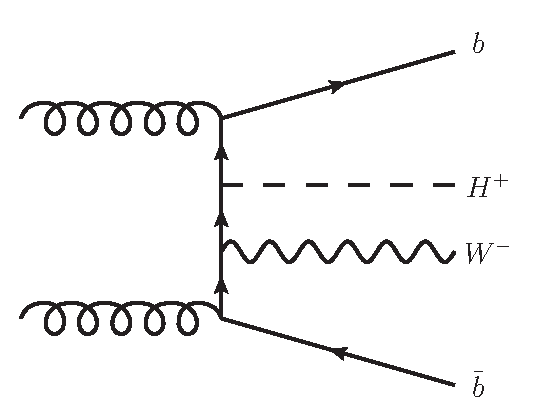
\includegraphics[width=0.3\linewidth]{chapters/chapter2_theory/images/NonResonant.pdf}}
		\subfloat[\label{fig:hpm-diagrams_b}]{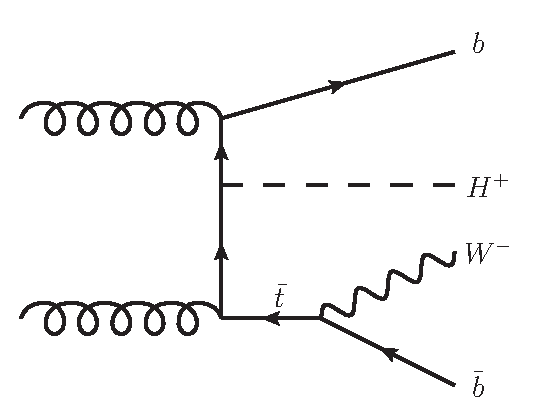
\includegraphics[width=0.3\linewidth]{chapters/chapter2_theory/images/SingleResonant.pdf}}
		\subfloat[\label{fig:hpm-diagrams_c}]{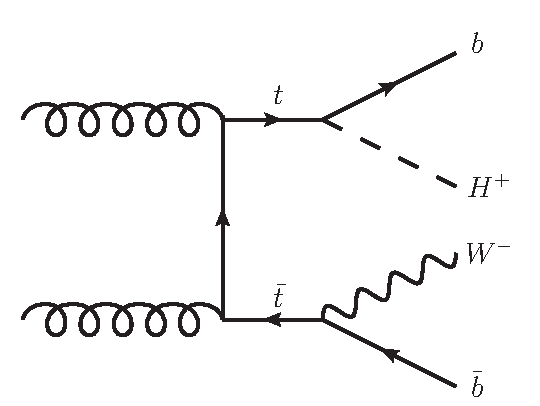
\includegraphics[width=0.3\linewidth]{chapters/chapter2_theory/images/DoubleResonant.pdf}}
		\caption{\label{fig:hpm-diagrams} Examples of leading-order Feynman diagrams contributing to the production of 
		charged Higgs bosons in $pp$ collisions: (a) non-resonant top-quark production, (b) single-resonant 
		top-quark production that dominates at large \Hpm masses, (c) double-resonant top-quark production that 
		dominates at low \Hpm masses. The interference between these three main diagrams becomes 
		most relevant in the intermediate-mass region.}
	\end{figure}
	\begin{figure}[!ht]
		\centering
		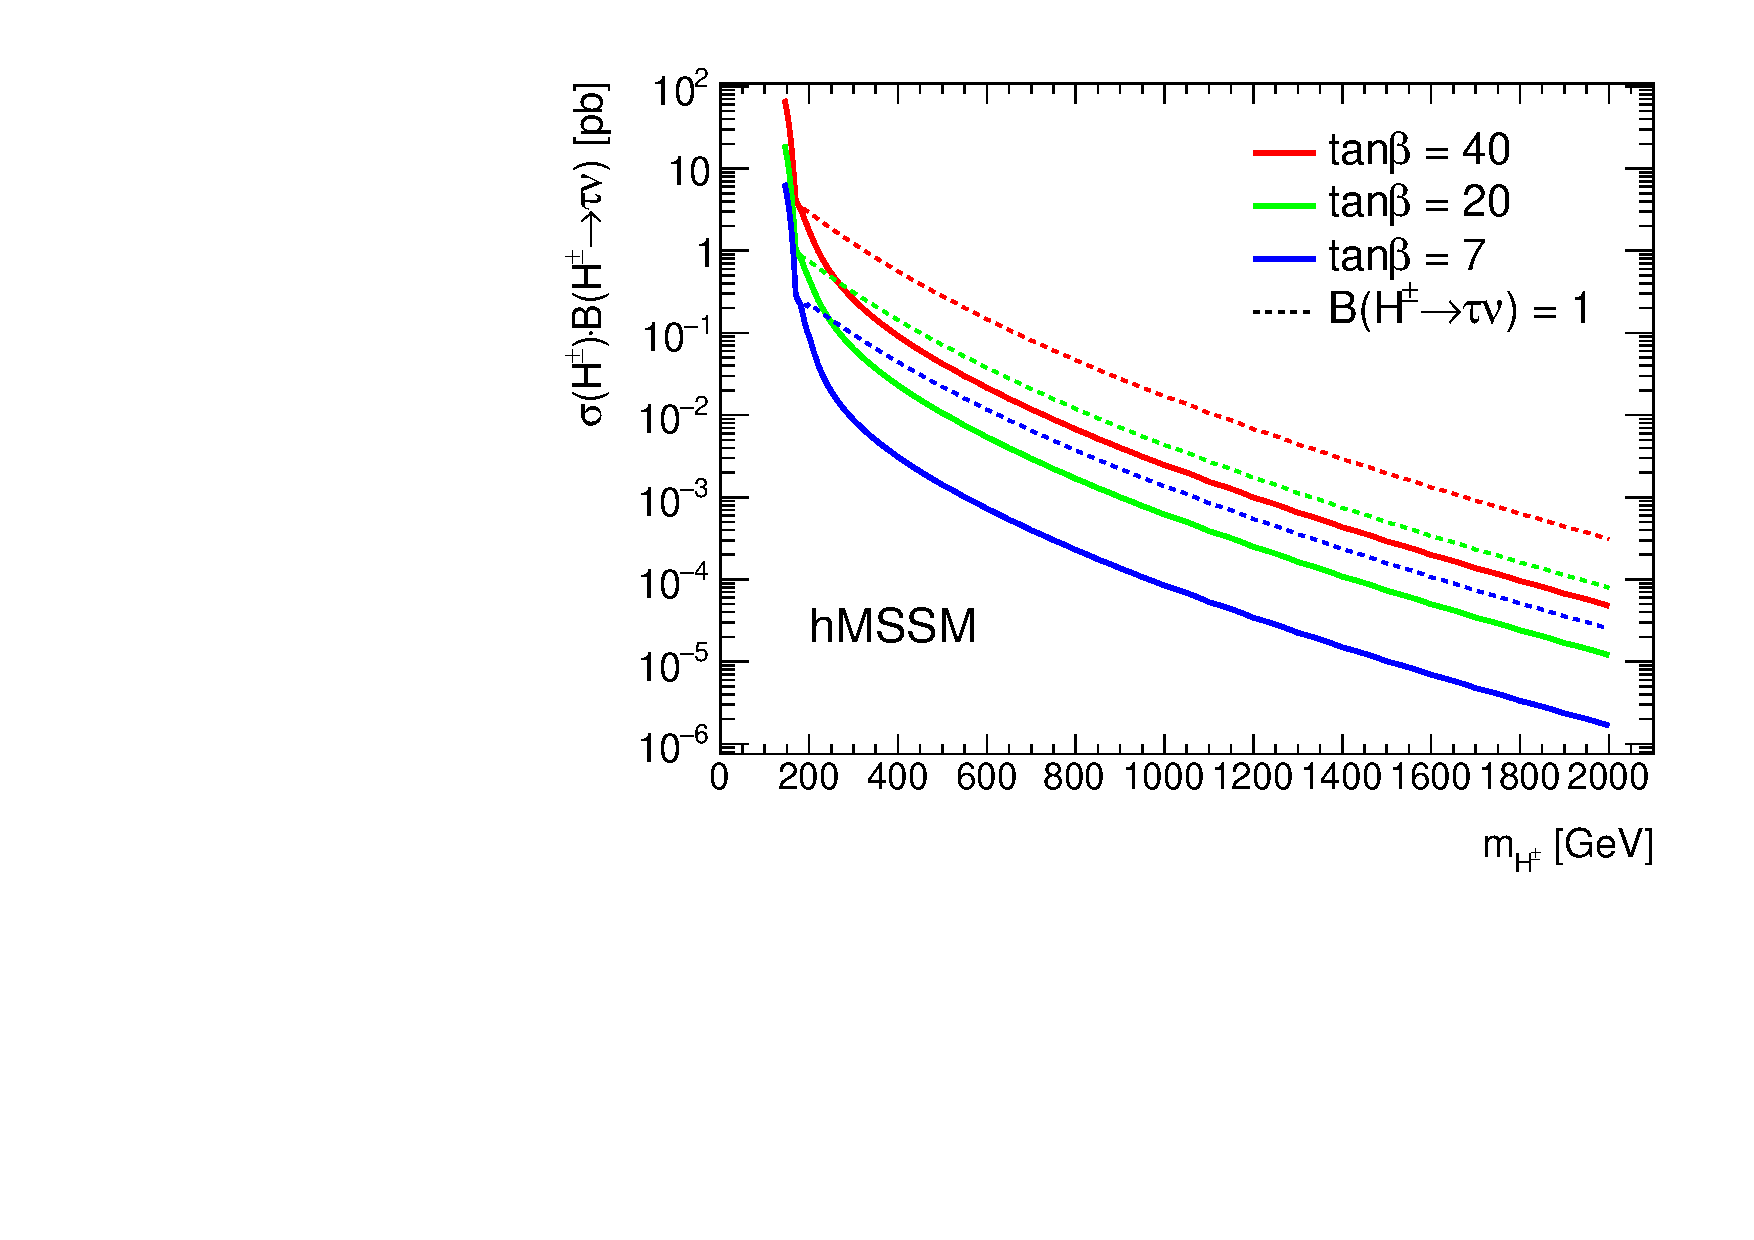
\includegraphics[width=0.75\linewidth]{chapters/chapter2_theory/images/XSBR_hmssm.pdf}
		\caption{\label{fig:hpm-xsec} Cross section of \Hpm at various \tanb values.}
	\end{figure}
	The production diagrams considered in this dissertation can be seen in figure \ref{fig:hpm-diagrams}. The cross section at various \tanb values can be seen as a function of \mHpm in figure \ref{fig:hpm-xsec}. As \tanb goes to smaller values the \Hpm cross section become smaller and at very small values the top Yukawa couplings become non-perturbative, meaning they are highly unlikely to occur. In this dissertation the decay channel considered is \HpmLong. 
	\begin{figure}[!ht]
		\centering
		\subfloat[\label{fig:hpm-br_a}]{\includegraphics[width=0.5\linewidth]{chapters/chapter2_theory/images/YRHXS3_BR_fig33.eps}}
		\subfloat[\label{fig:hpm-br_b}]{\includegraphics[width=0.5\linewidth]{chapters/chapter2_theory/images/YRHXS3_BR_fig34.eps}}
		\caption{\label{fig:hpm-br} Branching ratios of \Hpm for (a) $\tanb = 10$ and (b) $\tanb = 50$ ~\cite{Heinemeyer:2013tqa} }
	\end{figure}
	As can be seen in figure \ref{fig:hpm-br}, the \HpmLong decay channel is especially relevant at low \mHpm and high \tanb. The search described in this dissertation consists of two sub-channels, \taujets and \taulep, where the associated top decays either hadronically or leptonically respectively. 

	\subsection{Previous Result}\label{ssec:Prev Hpm}
		To add context to this dissertation, it is important to reference the results of the previous iteration of the search discussed in this dissertation. The ATLAS collaboration published a paper in 2018 covering the data taking years of 2015 and 2016 \cite{hpm-previous}, whereas this dissertation covers the full Run-2 (2015-2018) dataset. 
		\begin{figure}[!ht]
			\centering
			\subfloat[\label{fig:hpm-prev-limits_a}]{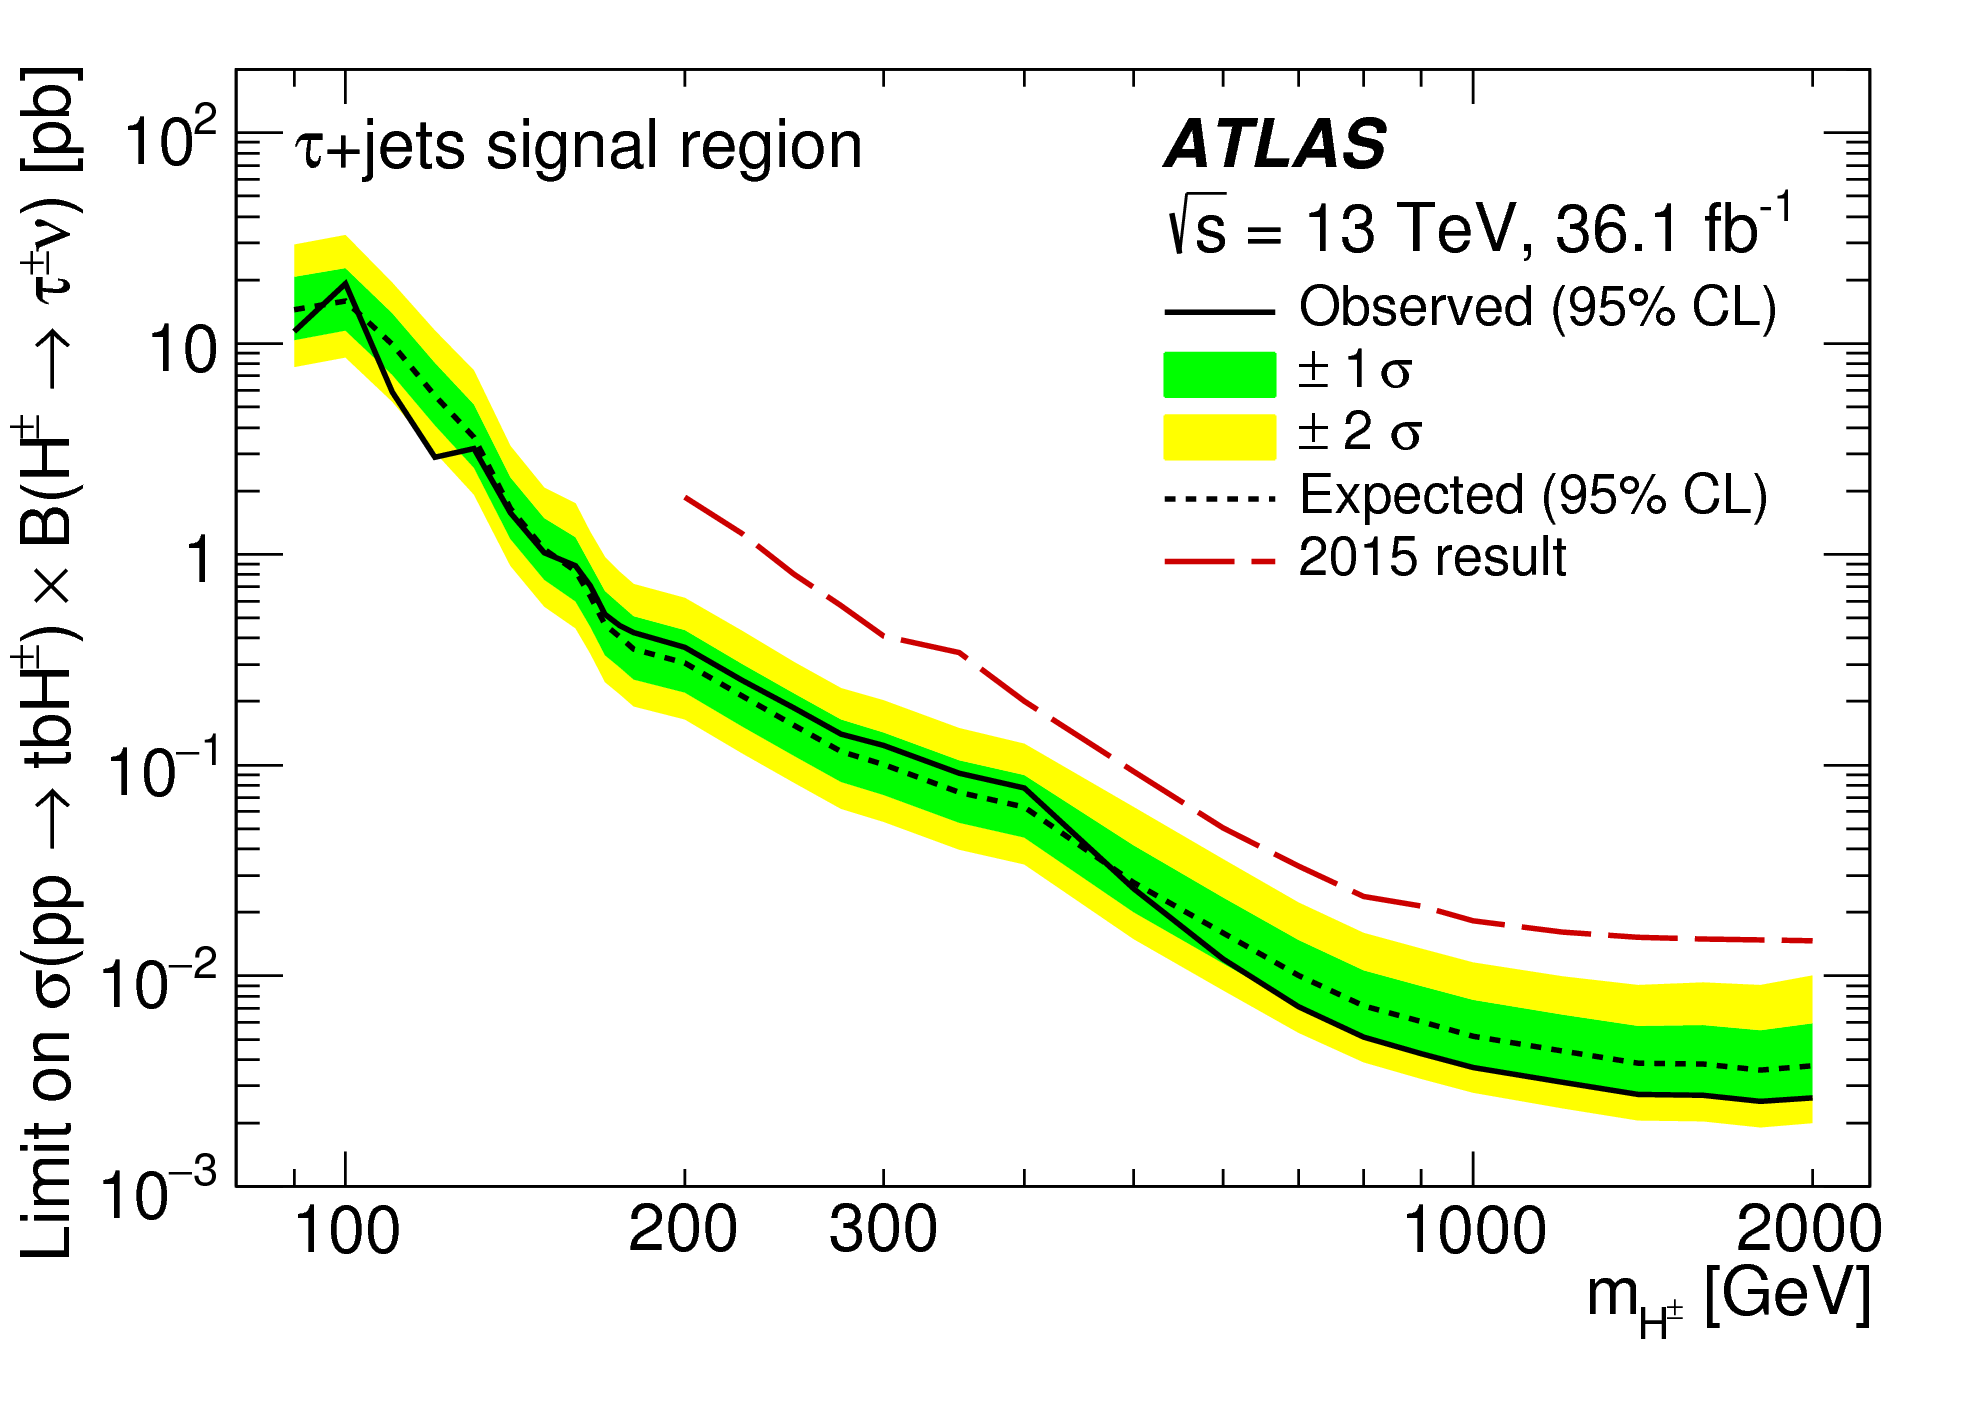
\includegraphics[width=0.5\linewidth]{chapters/chapter2_theory/images/Previous_Limits_Taujets.png}}
			\subfloat[\label{fig:hpm-prev-limits_b}]{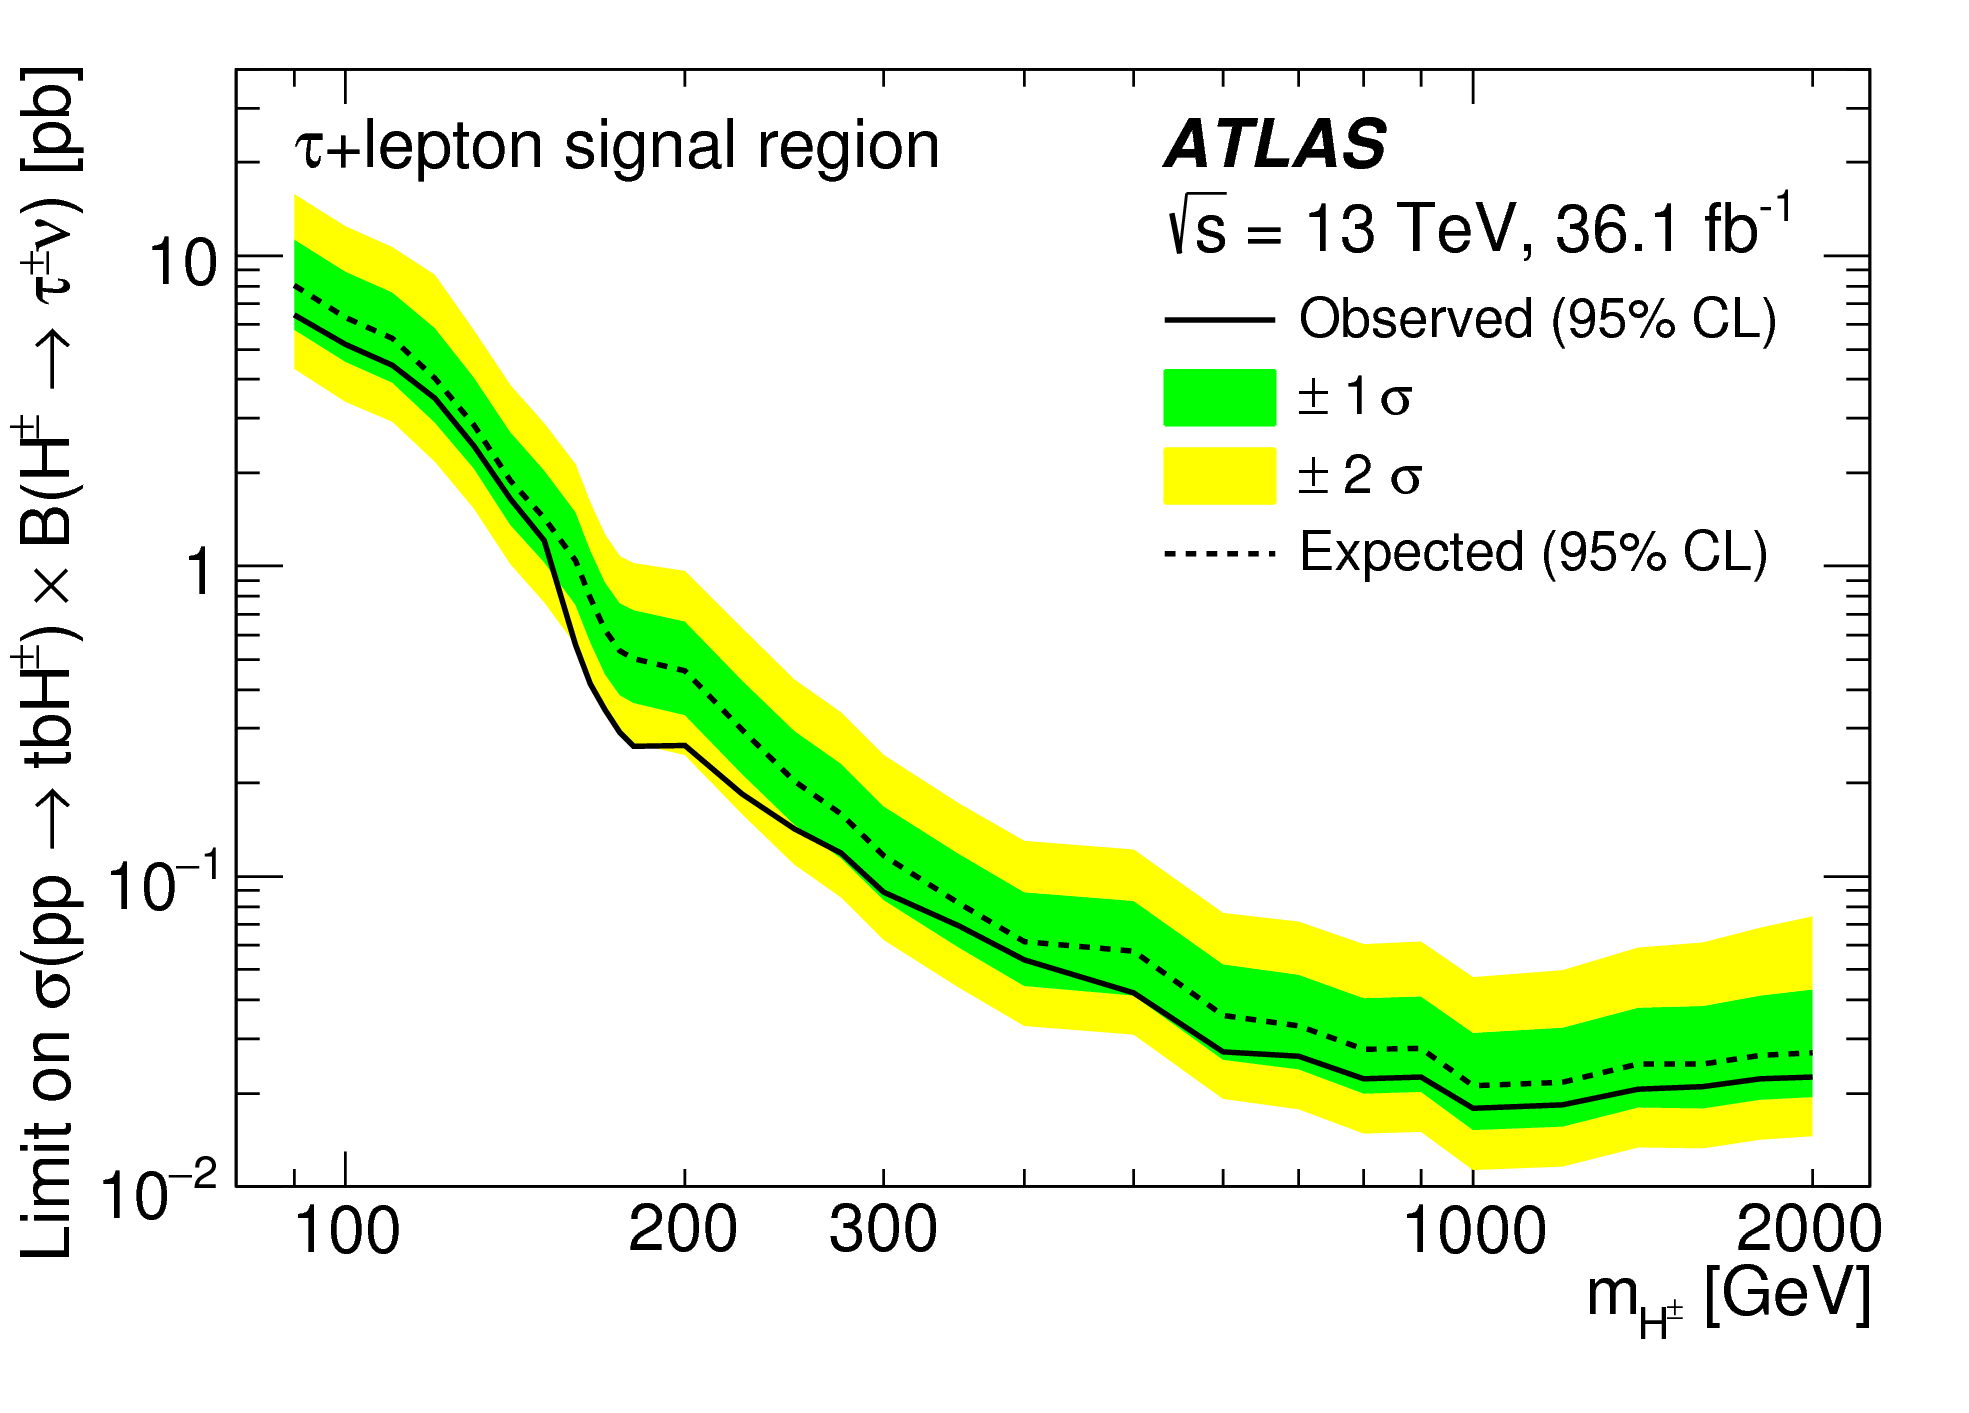
\includegraphics[width=0.5\linewidth]{chapters/chapter2_theory/images/Previous_Limits_Taulep.png}} \\
			\subfloat[\label{fig:hpm-prev-limits_c}]{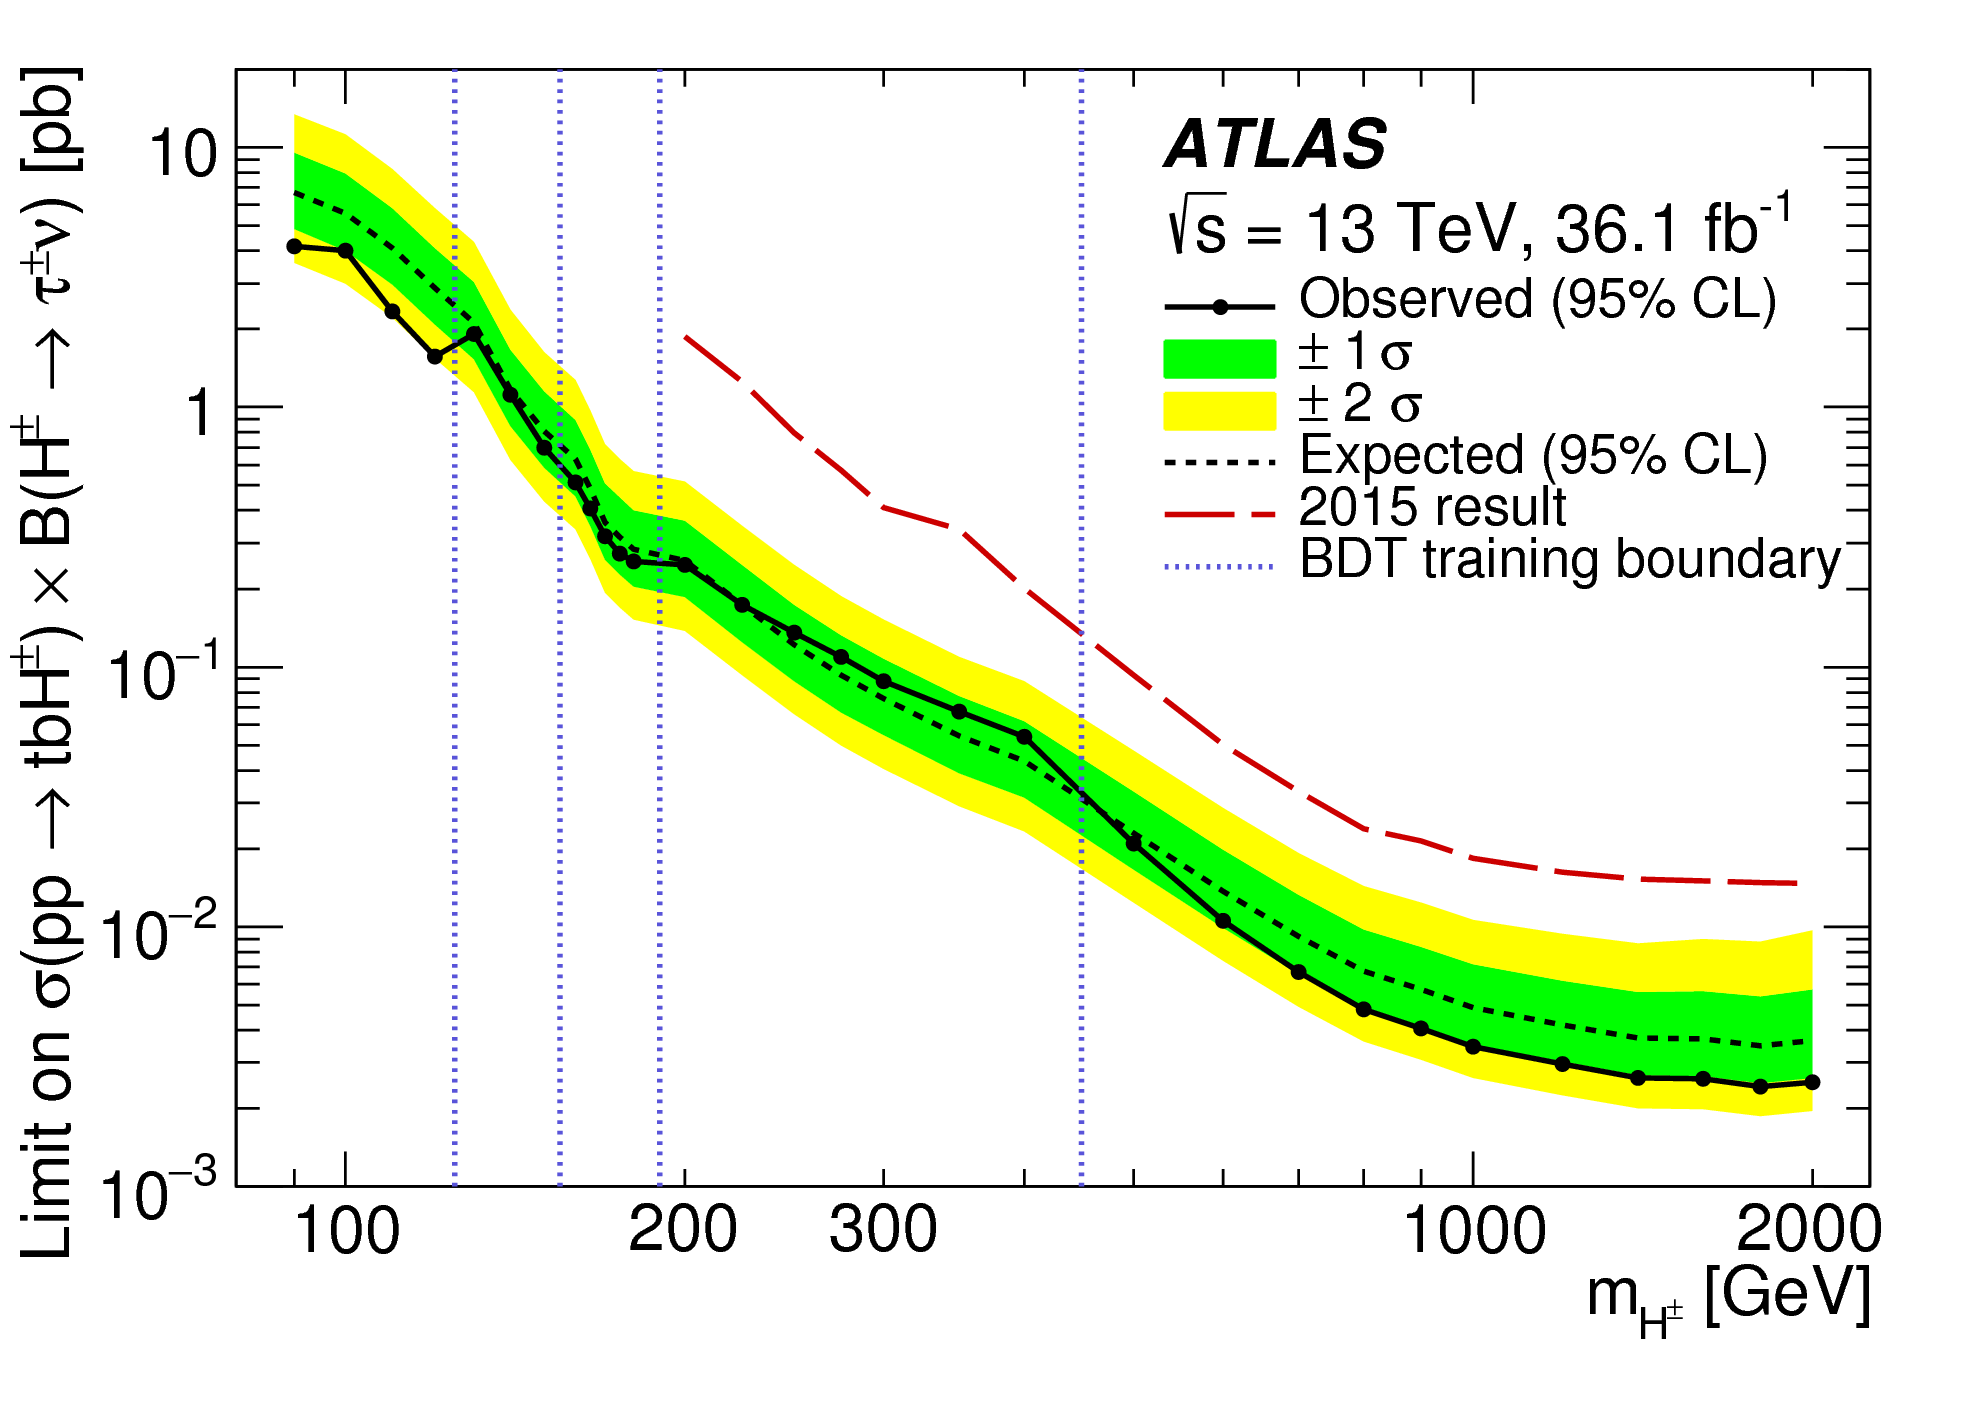
\includegraphics[width=0.75\linewidth]{chapters/chapter2_theory/images/Previous_Limits_Combined.png}}
			\caption{\label{fig:hpm-prev-limits} Limits on $\sigma(pp \rightarrow tbH^{\pm} x B(H^{\pm} \rightarrow \tau^\pm \nu)) [pb]$. (a) is for the \taujets subchannel (b) corresponds to the \taulep subchannel and (c) is the combination of the two subchannels. \cite{hpm-previous} }
		\end{figure}
		\begin{figure}[!ht]
			\centering
			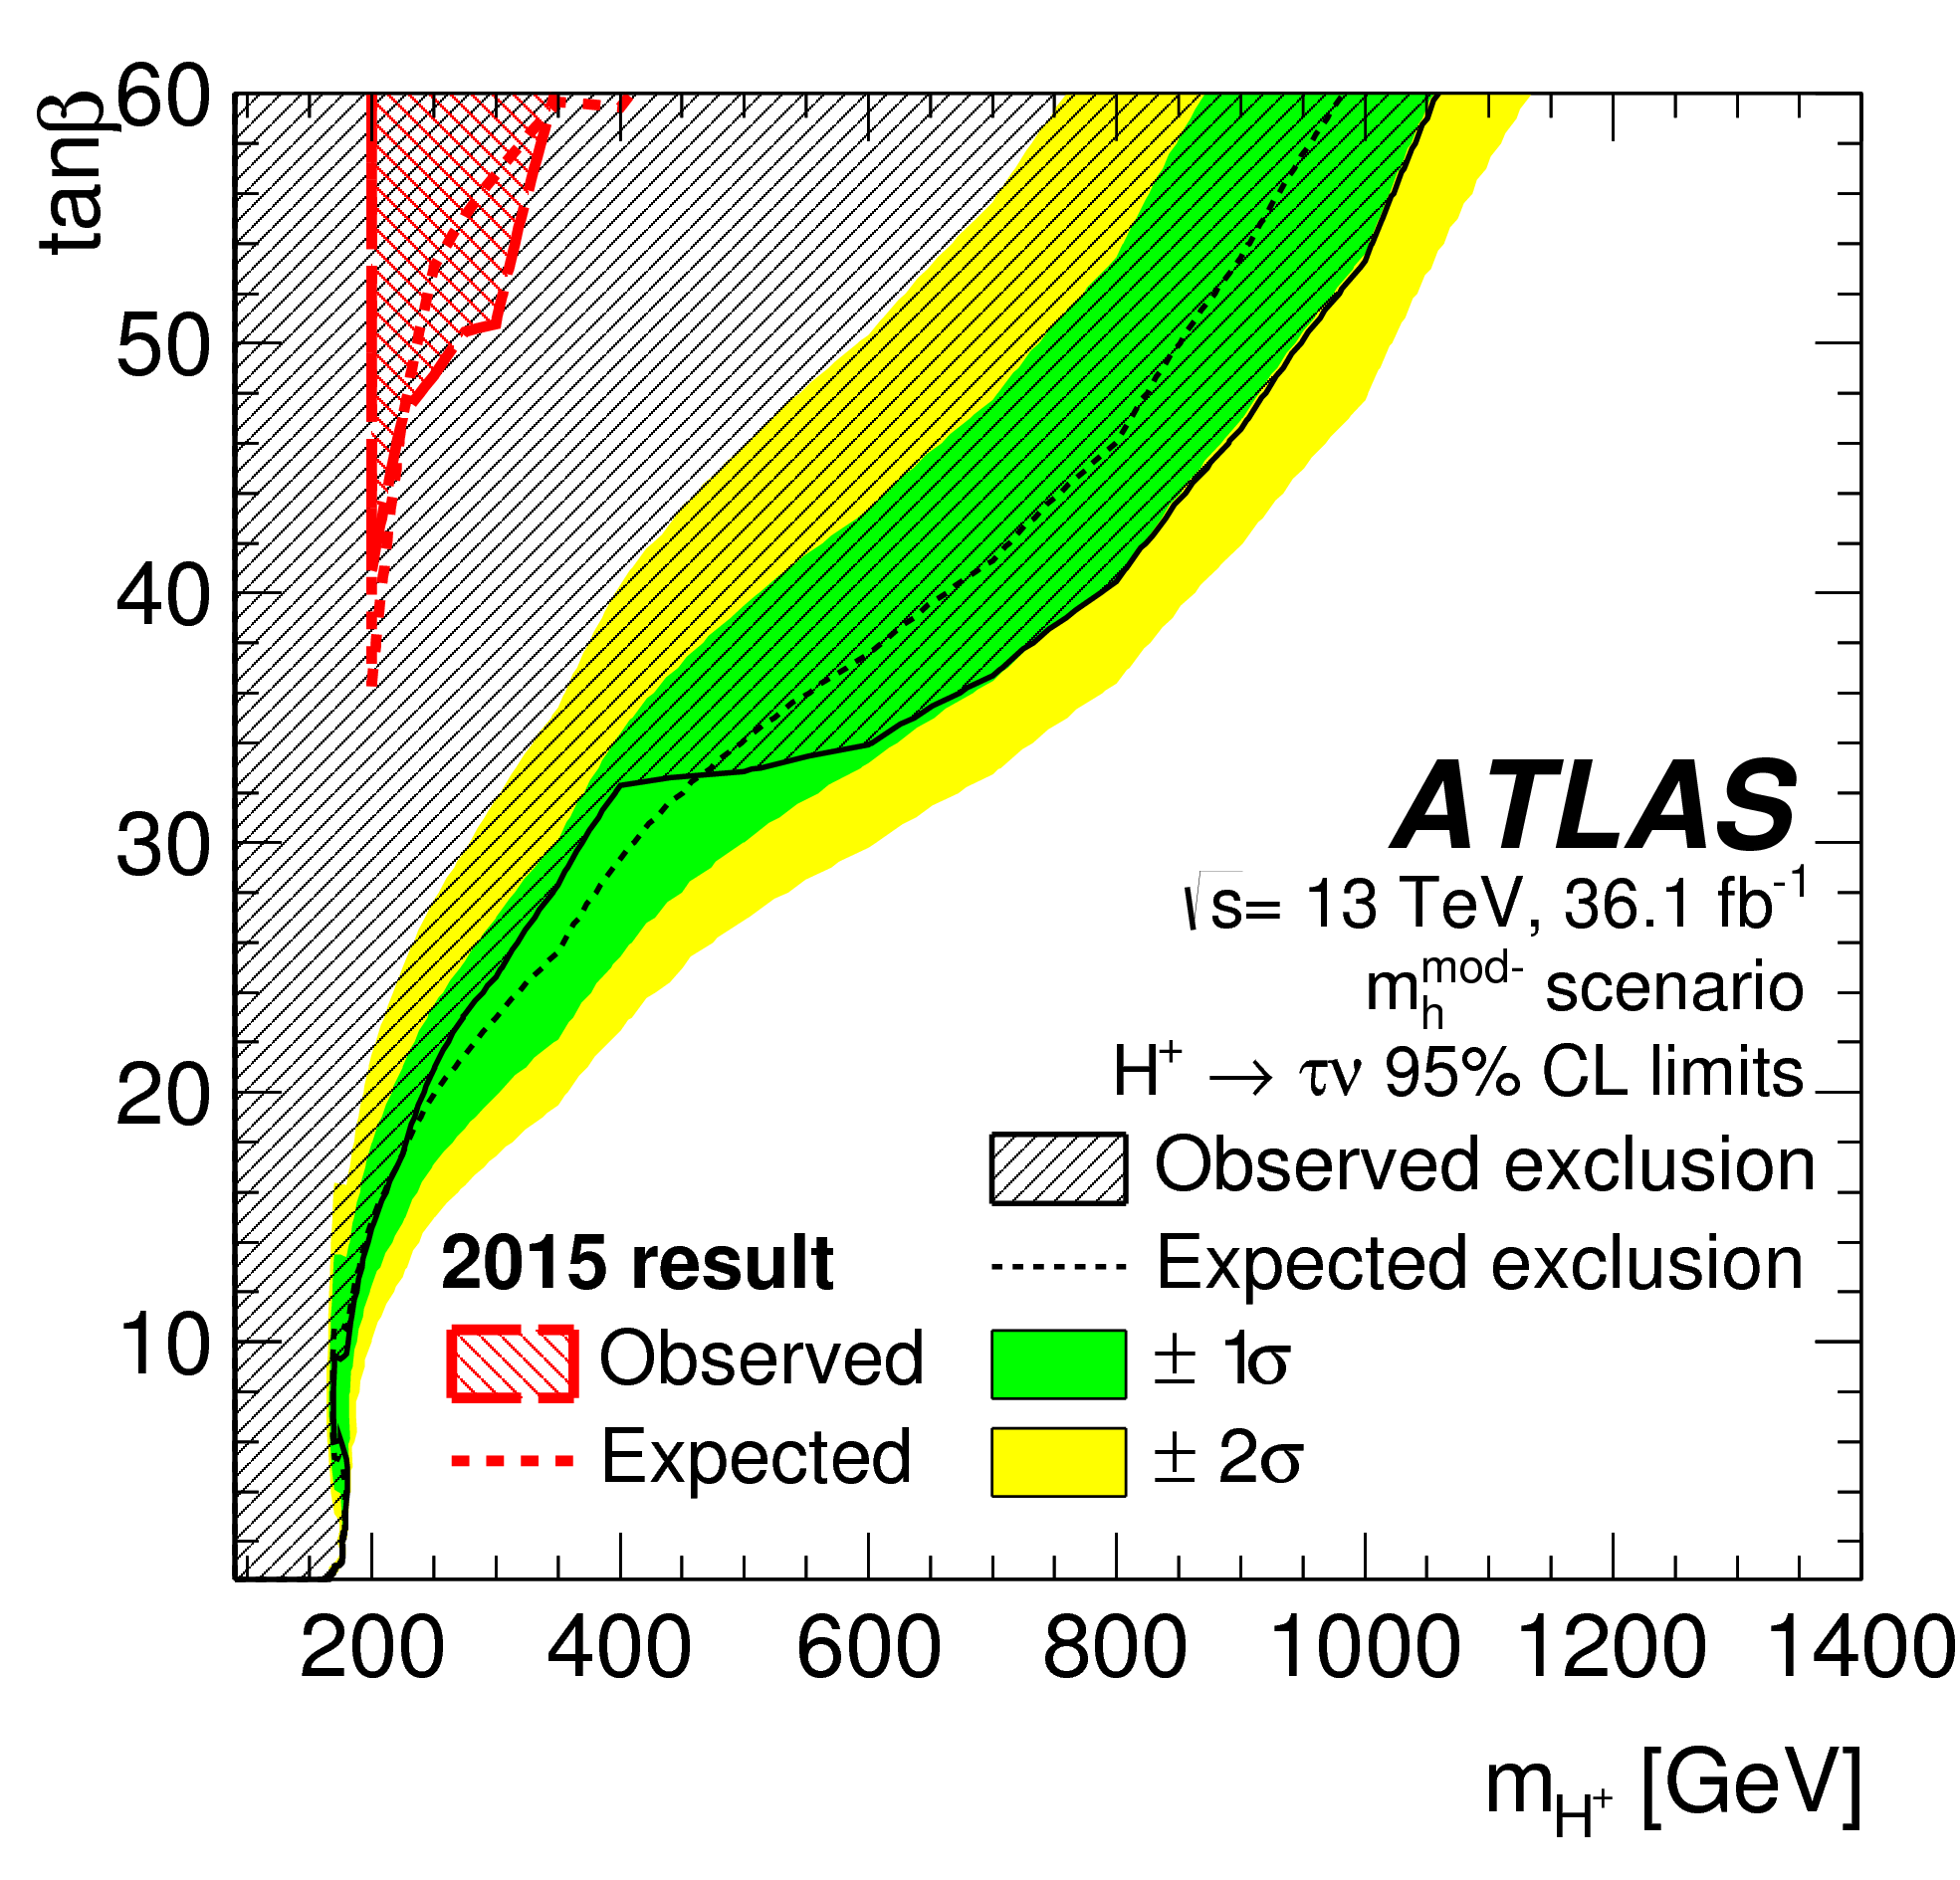
\includegraphics[width=0.75\linewidth]{chapters/chapter2_theory/images/Previous_Limits_Combined_tanb.png}
			\caption{\label{fig:hpm-prev-limits-tanb} Limits on \tanb as a function of \mHpm. \cite{hpm-previous} }
		\end{figure}
		Figure \ref{fig:hpm-prev-limits} shows the limits on the cross section and figure \ref{fig:hpm-prev-limits-tanb} shows the limits on \tanb as a function of \mHpm. 

		The previous iteration of this analysis used boosted decision trees (BDT) binned in \mHpm, giving them five separate classifiers to cover the mass range of $90 - 2000$ GeV. The mass bins can be seen as the blue dotted lines in Figure \ref{fig:hpm-prev-limits_c}. It is important to note the inclusion of the mass range $90 - 200$ GeV, as \cite{hpm-previous} was the first search to include this mass region below the top quark mass of $175$ GeV.